\documentclass{jsreport}
\usepackage{graphicx, url, algorithm, algorithmic, float, booktabs, listings, color, pdfpages, amsmath, amssymb, latexsym, mathtools, ascmac, amsfonts, amsthm}
\lstset{
  basicstyle={\ttfamily},
  identifierstyle={\small},
  commentstyle={\smallitshape},
  keywordstyle={\small\bfseries},
  ndkeywordstyle={\small},
  stringstyle={\small\ttfamily},
  frame={tb},
  breaklines=true,
  columns=[l]{fullflexible},
  numbers=left,
  xrightmargin=0zw,
  xleftmargin=3zw,
  numberstyle={\scriptsize},
  stepnumber=1,
  numbersep=1zw,
  lineskip=-0.5ex
}
\usepackage[table,xcdraw]{xcolor}
\newtheorem{theo}{定理}[chapter]
\newtheorem{defi}{定義}[chapter]
\newtheorem{lemm}{補題}[chapter]
\newtheorem{prop}{命題}[chapter]
\newtheorem{coro}{系}[chapter]
\newcommand{\red}[1]{\textcolor{red}{#1}}
\newcommand{\blue}[1]{\textcolor{blue}{#1}}
\newcommand{\green}[1]{\textcolor{green}{#1}}
\renewcommand{\baselinestretch}{1.1}
\usepackage{mathrsfs}
\usepackage{bm}
\def\qed{\hfill $\Box$}
\usepackage{tikz}
\usetikzlibrary{intersections, calc, arrows}
\renewcommand\proofname{\bf 証明}

\begin{document}
\chapter{確率変数と確率分布}
\section{母集団と標本}
既知の無作為標本によって母集団の未知の性質を知ろうとすることを統計的推測 (statistical inference) という (図\ref{fig:inf}).
\begin{figure}[htb]
  \centering
  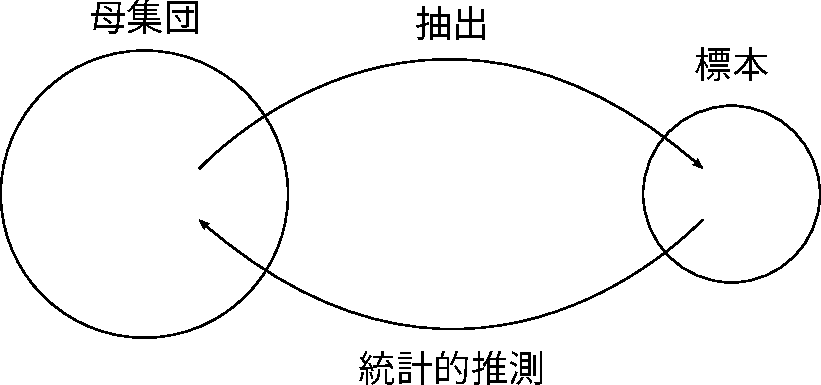
\includegraphics[clip, width=8cm]{../figure/infer.pdf}
  \caption{統計的推測のイメージ}
  \label{fig:inf}
\end{figure}

\section{確率変数と確率分布}
\subsection{確率変数}
まず,離散型の確率変数とその分布を考える.$X$を2個のサイコロを投げたときに出た目の和を表す変数とする (表\ref{tab:ex_pr}).
\begin{table}[htb]
  \centering
  \caption{確率変数の例}
  \begin{tabular}{c|ccccc|c}
    $X$の値 & $2$ & $3$ & $4$ & $\cdots$ & $12$ & 計 \\ \hline
    確率 & $1/36$ & $2/36$ & $3/36$ & $\cdots$ & $1/36$ & $1$ \\ \hline
  \end{tabular}
  \label{tab:ex_pr}
\end{table}

この$X$のように,取りうる値に対して,確率が対応する変数を確率変数 (random variable) と呼ぶ.確率変数の取りうる値 (実現値) とその確率をペアにしたものを確率分布 (probability distribution) と呼ぶ.

\begin{screen}
  \begin{defi}[分布関数]
    確率変数$X$の分布関数 (distribution function) を
    \begin{equation}
      F(x) = P(X \leq x) \nonumber
    \end{equation}
    によって定義する.
  \end{defi}
\end{screen}

分布関数$F(\cdot)$は以下の性質を持つ.
\begin{description}
  \item[(DF1)] 任意の$x \in \mathbb{R}^1$に対して,$0 \leq F(x) \leq 1$であり,かつ,
  \begin{equation}
    F(-\infty) \coloneqq \lim_{x \to -\infty} F(x) = 0, \; \; F(\infty) \coloneqq \lim_{x \to \infty} F(x) = 1. \nonumber
  \end{equation}
  \item[(DF2)] $F(x)$は単調非減少である : $x < y \Longrightarrow F(x) \leq F(y).$
  \item[(DF3)] $F(x)$は右側連続である : $\lim_{y \to x + 0} F(y) = F(x).$
\end{description}
逆に,これらの性質を持つものを分布関数として定義してもよい.

確率変数$X$の分布関数が$F(x)$である場合に,「確率変数$X$は分布$F(\cdot)$に従う」といい,``$X \sim F$''と書くことがある.

\begin{screen}
  \begin{defi}[離散分布]
    確率変数$X$の実現値が有限個または可算無限個の値の離散値
    $x_1, x_2, \ldots, x_n, \ldots$のみをとるとき,離散型確率変数といい,その分布を離散分布 (discrete distribution) という.
    各値$x_i$に対する確率を$p_i$とすると,離散分布は
    \begin{equation}
      f_k = f(x_k) = P(X = x_k) = p_k \; \; (k = 1, 2, \ldots)
    \end{equation}
    である.つまり,離散分布は各値に対する確率によって決定される.
    ただし,$\sum_{k = 1}^{\infty} p_k = 1, \, p_k \geq 0 \; (k = 1, 2, \ldots)$である.
    $f(\cdot)$を確率関数 (probability function) という.
  \end{defi}
\end{screen}
ただし,以下の点に注意する.
\begin{enumerate}
  \item $\mathscr{X} = \{x_1, x_2, \ldots\}$を標本空間 (sample space) という.
  \item $P(X = x_k)$は,確率変数$X$が$x_k$をとる確率を意味する.
  \item 確率変数は大文字 (ex. $X$),実現値は小文字 (ex. $x$) で表す.
  \item 確率変数$X$の実現値が離散的なとき,離散型確率変数と呼ぶ.
\end{enumerate}

確率関数$f(\cdot)$は次の性質を満たす.
\begin{description}
  \item[(PF1)] $f(x_k) \geq 0$.
  \item[(PF2)] $\sum_{k = 1}^{\infty} f(x_i) = 1$.
  \item[(PF3)] 分布関数は$F(x) = \sum_{\{i: x_i \leq x\}} f(x_i).$
  \begin{itemize}
    \item $P(X = x_k) = F(x_k) - F(x_{k-1})$.
  \end{itemize}
\end{description}
逆に,これらの性質をもつものを確率関数と定義してもよい.図\ref{fig:dis}に確率変数が離散の場合の確率関数および分布関数を示す.

\begin{figure}[htb]
  \begin{minipage}[b]{0.5\linewidth}
    \centering
    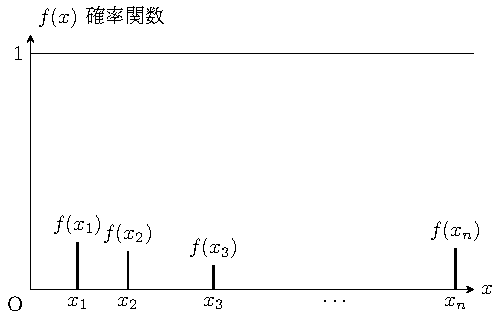
\includegraphics[clip, width=6cm]{../figure/dpf.pdf}
    \subcaption{確率関数}\label{fig:dpf}
  \end{minipage}
  \begin{minipage}[b]{0.5\linewidth}
    \centering
    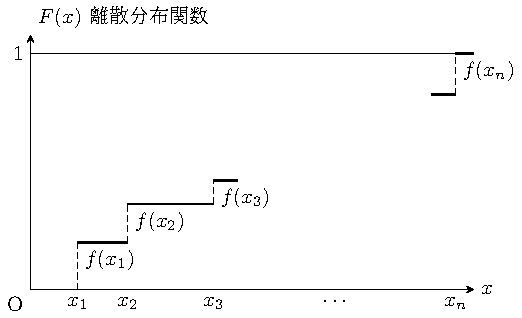
\includegraphics[clip, width=6cm]{../figure/dpdf.pdf}
    \subcaption{離散分布関数}\label{fig:dpdf}
  \end{minipage}
  \caption{確率関数および離散分布関数}\label{fig:dis}
\end{figure}

次に,連続型の確率変数と分布について定義する.

\begin{screen}
  \begin{defi}[連続分布]
    確率変数$X$が連続的な値をとるとき,連続型確率変数といい,その分布を連続分布 (continuous distribution) という.
    連続分布の分布関数が$C^1$級である時,その導関数
    \begin{equation}
      f(x) = \frac{dF(x)}{dx} \nonumber
    \end{equation}
    を$X$の確率密度関数 (probability density function) という.
  \end{defi}
\end{screen}

確率密度関数$f(\cdot)$は次の性質を満たす.
\begin{description}
  \item[(Dn1)] $f(x) \geq 0$.
  \item[(Dn2)] $\int_{-\infty}^{\infty} f(x) dx = 1$.
  \item[(Dn3)] 分布関数は$F(x) = \int_{-\infty}^x f(y) dy$.
  \begin{itemize}
    \item $P(a \leq X \leq b) = \int_{a}^b f(x) dx$
  \end{itemize}
\end{description}
逆にこれらの性質をもつものを確率密度関数と定義してもよい.連続型確率変数の1点における確率はゼロである.図\ref{fig:con}に確率変数が連続の場合の確率密度関数および分布関数を示す.
\begin{figure}[htb]
  \begin{minipage}[b]{0.5\linewidth}
    \centering
    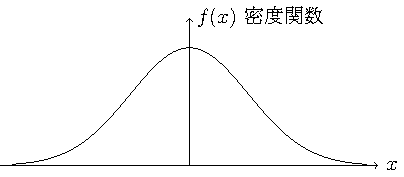
\includegraphics[clip, width=6cm]{../figure/cpf.pdf}
    \subcaption{確率密度関数}\label{fig:cpf}
  \end{minipage}
  \begin{minipage}[b]{0.5\linewidth}
    \centering
    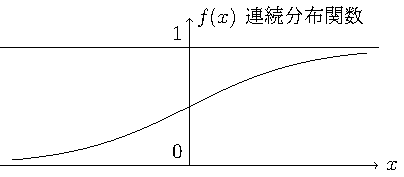
\includegraphics[clip, width=6cm]{../figure/cpdf.pdf}
    \subcaption{連続分布関数}\label{fig:cpdf}
  \end{minipage}
  \caption{確率密度関数および連続分布関数}\label{fig:con}
\end{figure}

確率変数をr.v.,確率密度関数をp.d.f.と略記することもある.
\section{分布の特性値 : 平均値と分散}
\begin{screen}
  \begin{defi}[平均値]
    \begin{enumerate}
      \item $X$が離散型確率変数のとき($P(X=x_i) = p_i \; (i = 1, 2, \ldots)$)

      $X$の平均値$E[X]$は,
      \begin{equation}
        E[X] \coloneqq \sum_{i = 1}^{\infty} x_i p_i \nonumber
      \end{equation}
      とする.
      \item $X$が連続型確率変数のとき($P(a \leq X \leq b) = \int_{a}^b f(x) dx$)

      $X$の平均値$E[X]$は,
      \begin{equation}
        E[X] \coloneqq \int_{-\infty}^{\infty} x f(x) dx \left(=\int_{-\infty}^{\infty} x dF(x)\right) \nonumber
      \end{equation}
    \end{enumerate}
  \end{defi}
\end{screen}

\begin{screen}
  \begin{defi}
    $h(X)$を連続関数として,$Y = h(X)$となる確率変数を考える.
    \begin{enumerate}
      \item $X$が離散型確率変数のとき
      \begin{equation}
        E[Y] = E[h(X)] \coloneqq \sum_{i=1}^{\infty} h(x_i)p_i \nonumber
      \end{equation}
      \item $X$が連続型確率変数のとき
      \begin{equation}
        E[Y] = E[h(X)] \coloneqq \int_{-\infty}^{\infty} h(x)f(x) dx \nonumber
      \end{equation}
    \end{enumerate}
  \end{defi}
\end{screen}

期待値は,以下の性質を持つ.
\begin{description}
  \item[(E1)] $c$を定数とすると,$E[c] = c$
  \item[(E2)] $X, Y$を確率変数,$h(X), k(X)$を連続関数,$a,b$を定数とする.
  \begin{equation}
    E[ah(X) + bk(Y)] = aE[h(X)] + bE[k(Y)] \nonumber
  \end{equation}
  \item[(E3)] $h(X) \geq 0 \Longrightarrow E[h(X)] \geq 0$
  \item[(E4)] $|E[h(X)]| \leq E[|h(X)|]$
\end{description}

\begin{screen}
  \begin{defi}[分散]
    $X$を確率変数とし,$E[X] = \mu, \, E[X^2] < \infty$とする.このとき,$X$の分散$V[X]$を
    \begin{equation}
      V[X] \coloneqq E[(X - E[X])^2] = E[(X - \mu)^2] \nonumber
    \end{equation}
    と定義する.また,標準偏差を$D[X] = \sqrt{V[X]}$と定義する.
  \end{defi}
\end{screen}

分散は,以下の性質を持つ.$X$を確率変数,$E[X] = \mu, \, E[X^2] < \infty$とし,$a, b$を定数とすると,
\begin{description}
  \item[(V1)] $V[X] = E[X^2] - \mu^2$
  \item[(V2)] $V[aX + b] = a^2V[X]$
\end{description}

(V1)について,
\begin{align}
  V[X] &= E[(X-E[X])^2] = E[(X - \mu)^2] \nonumber \\
  &= E[X^2 - 2E[X]\mu + \mu^2] = E[X^2] - \mu^2 \nonumber
\end{align}
である.

(V2)について,
\begin{align}
  V[aX + b] &= E[(aX + b - E[aX + b])^2] \nonumber \\
  &= E[(aX + b - aE[X] -b)^2] = E[a^2(X - E[X])^2] \nonumber \\
  &= a^2 E[(X - E[X])^2] = a^2 V[X] \nonumber
\end{align}
である.

\section{分布関数の変換}
確率分布は分布関数
\begin{equation}
  F(x) = \begin{cases}
    \sum_{x_k \leq x} P(X = x_k) & (離散型) \\
    \int_{-\infty}^x f(t)dt & (連続型)
\end{cases}\nonumber
\end{equation}
として与えられる.
関数のままでは分布の特徴をうまく表現できない.そこで,確率分布を扱いやすい関数に変換する.モーメントを特性値として捉える.

\begin{enumerate}
  \item 確率母関数 (probability generating function, p.g.f.)

  $X$: 離散型確率変数 ($x = 0, 1, 2, \ldots$)
  \begin{equation}
    P(t) \coloneqq E[t^X] = \sum_{x = 0}^{\infty} t^x P(X = x), \; |t| \leq 1 \nonumber
  \end{equation}
  を$X$の確率母関数という.
  \item 積率母関数 (moment generating function, m.g.f.)

  $X$: 確率変数
  \begin{equation}
    M(t) \coloneqq E[e^{tX}] = \begin{cases}
      \sum_{x = 0}^{\infty} e^{tx} P(X = x) & (離散型) \\
      \int_{-\infty}^{\infty} e^{tx} f(x) dx & (連続型)
  \end{cases} \nonumber
  \end{equation}
  を$X$の積率母関数という.
  \item 特性関数 (characteristic function, c.f.)

  $X$: 確率変数
  \begin{equation}
    \phi(t) \coloneqq E[e^{itX}] = \begin{cases}
      \sum_{x = 0}^{\infty} e^{itx} P(X = x) & (離散型) \\
      \int_{-\infty}^{\infty} e^{itx} f(x) dx & (連続型)
  \end{cases} \nonumber
  \end{equation}
  を$X$の特性関数という.
\end{enumerate}

ただし,以下の性質が成り立つ.
\begin{itemize}
  \item $X$が離散型確率変数のとき,$M(t) = P(e^t), \, \phi(t) = P(e^{it})$
  \item $M(t)$は一般に存在するとは限らないが,$\phi(t)$は常に存在する.
  \item $\phi(t) = M(it)$
\end{itemize}

モーメントの計算について,それぞれの関数は以下の性質が成り立つ.
\begin{description}
  \item[p.g.f.]
  $X$: 離散型確率変数, $E[X] < \infty, V[X] < \infty$
  \begin{align}
    \frac{dP(t)}{dt} &= \frac{d}{dt} \left(\sum_{x = 0}^{\infty} t^x P(X = x) \right) = \frac{d}{dt} \left(P(X = 0) + \sum_{x=1}^{\infty} t^x P(X = x)\right) \nonumber \\
    &= \sum_{x=1}^{\infty} \frac{d}{dt} (t^x P(X = x)) = \sum_{x = 1}^{\infty} x t^{x - 1} P(X = x) \nonumber
  \end{align}
  より,
  \begin{equation}
    \left.\frac{dP(t)}{dt}\right|_{t = 1} = \sum_{x = 1}^{\infty} xP(X = x) = \sum_{x = 0}^{\infty} xP(X = x) = E[X] \nonumber
  \end{equation}
  が成り立つ.同様にして,
  \begin{align}
    \frac{d^2P(t)}{dt^2} &= \frac{d}{dt} \left(\sum_{x = 1}^{\infty} x t^{x - 1} P(X = x)\right) = \frac{d}{dt} \left(P(X = 1) + \sum_{x = 2}^{\infty} xt^{x - 1} P(X = x)\right) \nonumber \\
    &= \sum_{x = 2}^{\infty} x(x - 1)t^{x - 2} P(X = x) \nonumber
  \end{align}
  より,
  \begin{equation}
    \left.\frac{d^2P(t)}{dt}\right| = \sum_{x = 2}^{\infty} x(x - 1)P(X = x) = \sum_{x = 0}^{\infty} x(x - 1)P(X = x) = E[X(X - 1)] \nonumber
  \end{equation}
  分散は,
  \begin{align}
    V[X] &= E[X^2] - (E[X])^2 = E[X(X - 1)] + E[X] - (E[X])^2 \nonumber \\
    &= \left.\frac{d^2 P(t)}{dt^2}\right|_{t = 1} + \left.\frac{d P(t)}{dt}\right|_{t = 1} - \left(\left.\frac{d P(t)}{dt}\right|_{t = 1}\right)^2 \nonumber
  \end{align}
  で求められる.

  \item[m.g.f.]
  $X$: (主に連続型)確率変数
  \begin{align}
    \frac{d M(t)}{dt} &= \frac{d}{dt} \left( \int_{-\infty}^{\infty} e^{tx} f(x) dx\right)
    = \int_{-\infty}^{\infty} \left(\frac{d}{dt} e^{tx}\right) f(x) dx \nonumber \\
    &= \int_{-\infty}^{\infty} x e^{tx} f(x) dx \nonumber
  \end{align}
  より,
  \begin{equation}
    \left.\frac{d M(t)}{dt}\right|_{t = 0} = \int_{-\infty}^{\infty} xf(x) dx = E[X]. \nonumber
  \end{equation}
  また,
  \begin{equation}
    \frac{d^2 M(t)}{dt^2} = \int_{-\infty}^{\infty} x^2 e^{tx} f(x) dx \nonumber
  \end{equation}
  より,
  \begin{equation}
    \left.\frac{d^2 M(t)}{dt^2}\right|_{t = 0} = \int_{-\infty}^{\infty} x^2 f(x) dx = E[X^2]. \nonumber
  \end{equation}
  よって,
  \begin{align}
    V[X] &= E[X^2] - (E[X])^2 \nonumber  \\
    &= \left.\frac{d^2 M(t)}{dt^2}\right|_{t = 0} - \left(\left.\frac{d M(t)}{dt}\right|_{t = 0}\right)^2. \nonumber
  \end{align}
  離散型確率変数についても同様.
  \item[c.f.]
  $E[X^2] < \infty$とする.
  m.g.f.と同様の議論により,
  \begin{equation}
    \left.\frac{d \phi(t)}{dt}\right|_{t = 0} = E[iX] = i E[X] \; \; \therefore E[X] = (-i) \left.\frac{d \phi(t)}{dt}\right|_{t = 0} \nonumber
  \end{equation}
  および
  \begin{equation}
    \left.\frac{d^2 \phi(t)}{dt^2}\right|_{t = 0} = E[-X^2] \; \; \therefore E[X^2] = - \left.\frac{d^2 \phi(t)}{dt^2}\right|_{t = 0} \nonumber
  \end{equation}
  が得られ,
  \begin{equation}
    V[X] = \left.\frac{d^2 \phi(t)}{dt^2}\right|_{t = 0} + \left(\left.\frac{d \phi(t)}{dt}\right|_{t = 0}\right)^2 \nonumber
  \end{equation}
  となる.
\end{description}

積率母関数の対数$\psi(t) = \log M(t)$をキュミュラント母関数 (cumulant generating function, c.g.f.) という.c.g.f.について,
\begin{equation}
  \frac{d \psi(t)}{dt} = \frac{M^{\prime}(t)}{M(t)}, \; \; \left.\frac{d \psi(t)}{dt}\right|_{t = 0} = \frac{M^{\prime}(0)}{M(0)}  = E[X] \nonumber
\end{equation}
および
\begin{equation}
  \frac{d^2 \psi(t)}{dt^2} = \frac{M(t) M^{\prime \prime}(t) - M^{\prime}(t)^2}{M(t)^2}, \; \; \left.\frac{d^2 \psi(t)}{dt^2}\right|_{t = 0} = \frac{E[X^2] - (E[X])^2}{1} = V[X] \nonumber
\end{equation}
が成り立つ.

以上はモーメントの計算について述べたが,確率分布の同値性および分布の収束について,以下の定理が成り立つ.

\begin{screen}
  \begin{theo}
    \begin{enumerate}
      \item 一致性
      \begin{description}
        \item[$X_1, X_2$] : 確率変数
        \item[$F_1, F_2$] : $X_1, X_2$の分布関数
        \item[$\phi_1, \phi_2$] : $X_1, X_2$の特性関数
      \end{description}
      とするとき,次が成立.
      \begin{equation}
        F_1 = F_2 \Longleftrightarrow \phi_1 = \phi_2 \nonumber
      \end{equation}
      \item 連続性
      \begin{description}
        \item[$X, X_n \, (n = 1, 2, \ldots)$] : 確率変数
        \item[$F, F_n \, (n = 1, 2, \ldots)$] : $X, X_n$の分布関数
        \item[$\phi, \phi_n \, (n = 1, 2, \ldots)$] : $X, X_n$の特性関数
      \end{description}
      とするとき,次が成立.
      \begin{equation}
        \lim_{n \to \infty} F_n(x) = F(x) \Longleftrightarrow \lim_{n \to \infty} \phi_n(t) = \phi(t) \nonumber
      \end{equation}
      が成り立つ.ただし,$x$は$F$の連続点,$t$は任意である.
    \end{enumerate}
  \end{theo}
\end{screen}

\end{document}
